\documentclass{article}
\usepackage{graphicx} % Required for inserting images
\usepackage{ntheorem}
\usepackage{verbatim}
\usepackage{float}
\usepackage{amsmath}
\usepackage{amsmath} 
\usepackage{amssymb}
\usepackage[style=authoryear,backend=biber,natbib=true,maxcitenames=2]{biblatex}
\usepackage[a4paper, total={6in, 8in}]{geometry}
\usepackage{xcolor}
\usepackage{subcaption}
\usepackage{hyperref}
\usepackage{booktabs}
% \usepackage[T1]{fontenc}
% \usepackage{imakeidx}
\makeindex
\hypersetup{colorlinks,linkcolor={blue},citecolor={blue},urlcolor={red}}  
% Custom commands
\newcommand{\D}{\mathcal{D}}
\newcommand{\W}{\mathcal{W}}
\renewcommand{\P}{\mathcal{P}}
\newcommand{\R}{\mathbb{R}}
\newcommand{\norm}[2]{\|{#1}\|_{#2}}
\renewcommand{\t}{^{\top}}



\theoremseparator{:}
\newtheorem{hyp}{Hypothesis}
\addbibresource{references.bib}
\title{Machine Learning \underline{Fairness} Under a Modern \\ Optimization Lens}
\author{Nicolás Acevedo Villena, Vasiliki Efthymiou}
\date{November 2025}






\begin{document}
\maketitle

\tableofcontents
\newpage

\section{Motivation}

Machine learning (ML) models are increasingly used to support or automate high-stakes decisions in various domains, including credit, hiring, healthcare, and public policy (see \cite{Sahoh2023}). In these settings, optimizing predictive accuracy alone is not sufficient: stakeholders also care about whether model outputs systematically disadvantage certain individuals or groups. As a result, \emph{fairness} constraints have become a central requirement for responsible ML deployment, alongside traditional considerations like accuracy, interpretability, privacy, and robustness (see \cite{Mehrabi2021}).
\begin{figure}[!h]
    \centering
    
\includegraphics[width=0.5\linewidth, trim={0 1cm 0 1cm}]{Fairness Price/MLOpt Project on Fairness/img/tradeoff_plot (1).pdf}
    \caption{Caption}
    \label{fig:tradeoff}
\end{figure}
A key difficulty is that fairness is inherently \emph{context-dependent}. Different applications, institutions, and legal frameworks can imply different (and sometimes incompatible) notions of fairness. For example, one may want to equalize error rates across protected groups, ensure that predictions are statistically independent of sensitive attributes, or avoid systematic regressivity in outcomes. This plurality of definitions means that fairness cannot be treated as a single universal scalar metric; rather, it is best viewed as a family of constraints and objectives that encode the values and requirements of a particular decision context. Further, the fairness measure are usually not even compatible with the accuracy of the model (e.g. \cite{Dutta2019ki}, \cite{Liu2020AccuracyAF}), as we can see in the \textit{tradeoff} curve between prediction error and unfairness in terms of pairwise difference of accuracy in Figure \ref{fig:tradeoff}.

% \subsection{Where does unfairness come from?}
Fairness concerns arise from multiple sources. Bias can be introduced by the data (e.g., underrepresentation, measurement error, historical inequities reflected in labels) and also by the learning algorithm itself (e.g., inductive biases and optimization choices that amplify disparities). Moreover, practical data issues such as missingness and distribution shift can disproportionately affect specific groups, making it possible for a model to appear fair on a training dataset while violating fairness desiderata after deployment. Therefore, addressing fairness requires an end-to-end perspective that goes beyond post-hoc evaluation.

These considerations motivate an \emph{optimization lens} on fairness in ML. Many fairness interventions can be naturally expressed as modifications to the learning problem:
\begin{itemize}
    \item[(i)] \emph{pre-processing} approaches that alter or reweight training data,
    \item[(ii)] \emph{in-processing} approaches that incorporate fairness directly into training via constraints, penalties, or multi-objective optimization (MOO) formulations, and
    \item[(iii)] \emph{post-processing} approaches that adjust outputs to satisfy fairness criteria.
\end{itemize}
Among these, in-processing and multi-objective perspectives are particularly attractive when fairness must be balanced against predictive performance and when multiple fairness desiderata are present simultaneously. Casting fairness as constraints or explicit objectives makes the trade-offs transparent and controllable, and it enables the use of modern optimization tools to analyze feasibility, sensitivity to hyperparameters, and the structure of the accuracy--fairness frontier.

Finally, in many realistic deployments, the sensitive attribute is available for auditing and model development, but may be restricted or undesirable to use at prediction time. This setting highlights a fundamental tension: we may want predictions that do not depend on sensitive attributes, yet we still need access to those attributes to \emph{measure} disparities and to \emph{enforce} fairness requirements during training. Overall, the goal is to develop learning formulations that make fairness a first-class design principle---yielding models that achieve strong predictive performance while satisfying application-relevant fairness requirements and providing interpretable trade-offs for decision makers.

\subsection{Project goals: A ``holistic" approach to fairness}

In more detail, we aim to study the behavior of the empirical and theoretical interplay between predictive power and multiple senses of fairness among different sensitive demographic groups on optimal and robust machine learning models, using pre-existing data sources available and already studied in the literature (see \cite{Martinez2022}). In particular:
\begin{enumerate}
    \item We examine whether optimal $ k$-Nearest Neighbors (KNN) imputation (\cite{JMLR:v18:17-073}) in a biased dataset with missing values can amplify the already present bias (\textit{pre-processing} approach).
    \item We analyze the behavior of fairness-constrained Stable Regression and a robust adversarial simile of it, and whether they can amplify or improve disparities across sensitive groups (\textit{in-processing} approach).
\end{enumerate}

In other words, we adopt a \textit{holistic} approach to fairness, examining both the role of the dataset itself and the predictive algorithm.

\section{Related Work}
\par \par There is a large body of work on detecting bias in datasets (e.g., \cite{engstrom2020identifyingstatisticalbiasdataset}) and on bias mitigation methods (e.g., \cite{jain2024datadebiasingdatamodelsd3m, celentano2023challengesinconsistencyregimenovel}, where the latter focuses specifically on bias mitigation in the presence of missing data). However, the problem of data imputation has largely been studied independently of the fairness and debiasing literature.
\par In addition, prior work suggests that robustness and fairness are not necessarily aligned. \citet{hashimoto2018fairness} and \citet{iosifidis2020fairness} show that robust objectives can either mitigate or exacerbate disparities, depending on the loss geometry and data imbalance. For instance, robust models may overweight high-loss samples, which often belong to majority groups if those groups dominate the training distribution. Similarly, stability-focused methods such as CVaR regression may ignore minority patterns if they appear as ``outliers.''

Despite this, there has been limited systematic analysis of how robustness interacts with fairness constraints or penalties. Some attempts to bridge this gap include fairness-aware DRO \citep{chiang2020fairness, wadsworth2018achieving}, adversarial reweighting \citep{zhang2018mitigating}, and regularization-based approaches that incorporate fairness as a penalty term. However, the trade-off frontier between robustness and fairness—how one affects the other in practical models—remains not completely understood.


% \section{Fairness Metrics}

% We consider several commonly used statistical measures of demographic group fairness as potential (un) fairness level metrics, each capturing a distinct notion of parity between sensitive groups. Let $A \in \{0,1\}$ denote the sensitive attribute (e.g., gender or race), $Y \in \{0,1\}$ the true label, and $\hat{Y} = \mathbb{I}\{\sigma(w^\top x) \ge \tau\}$ the predicted label, where $\sigma(\cdot)$ is the logistic function and $\tau$ is a threshold.

% \paragraph{Demographic Parity (DP).}
% A classifier satisfies demographic parity if its positive prediction rate is independent of the sensitive attribute:
% \begin{equation}
% \Pr(\hat{Y} = 1 \mid A = 0) = \Pr(\hat{Y} = 1 \mid A = 1).
% \end{equation}
% We measure deviations from this ideal by the \emph{DP gap}:
% \begin{equation}
% \Delta_{\text{DP}}(w) = \left| \Pr(\hat{Y} = 1 \mid A = 0) - \Pr(\hat{Y} = 1 \mid A = 1) \right|.
% \end{equation}

% \paragraph{Equalized Odds (EO).}
% Equalized odds requires predictions to be conditionally independent of $A$ given $Y$:
% \begin{equation}
% \Pr(\hat{Y} = 1 \mid A = 0, Y = y) = \Pr(\hat{Y} = 1 \mid A = 1, Y = y), \quad \forall y \in \{0,1\}.
% \end{equation}
% The corresponding \emph{EO gap} aggregates the conditional differences:
% \begin{equation}
% \Delta_{\text{EO}}(w) = \frac{1}{2} \sum_{y \in \{0,1\}} 
% \left| \Pr(\hat{Y} = 1 \mid A = 0, Y = y) - \Pr(\hat{Y} = 1 \mid A = 1, Y = y) \right|.
% \end{equation}

% \paragraph{Equal Opportunity (EOp).}
% A relaxed version of EO, equal opportunity enforces parity only for the truly positive class ($Y=1$):
% \begin{equation}
% \Pr(\hat{Y} = 1 \mid A = 0, Y = 1) = \Pr(\hat{Y} = 1 \mid A = 1, Y = 1).
% \end{equation}
% The \emph{EOp gap} is then defined as:
% \begin{equation}
% \Delta_{\text{EOp}}(w) = \left| \Pr(\hat{Y} = 1 \mid A = 0, Y = 1) - \Pr(\hat{Y} = 1 \mid A = 1, Y = 1) \right|.
% \end{equation}
% \paragraph{Implementation.}
% In practice, these probabilities are estimated empirically on the test data, and we use continuous relaxations by replacing $\hat{Y}$ with the predicted probability $\sigma(w^\top x)$ to obtain smooth, differentiable surrogates suitable for optimization.

% \section{Proposed Approach}

%    In robust optimization applied to machine learning, we train against the worst-case scenario for noise in our dataset. But in some cases, this may lead to a biased model in the sense that it favors one sensitive group. Similarly, in stable regression, the worst-case subset of training samples may also lead to favoritism for some group.  
%     \begin{itemize}
%         \item  Can we find empirical evidence that this happens? 
%         \item Can we address this problem with a combined optimization approach?
%         \item If not: Can we propose a general method that takes into account fairness and robustness as a whole?
%     \end{itemize}

% There is no clear answer to these questions, or the correct technique that improves both the generalization power and fairness of a predictive model. Hence, we analyze different alternatives as a potential project. These include:
% \begin{itemize}
%     \item Optimization of machine learning models with fairness constraint: Solve a classic minimization of loss function (and its robust form), and add (un) fairness constraints to the modeling.  
%     \item Treating fairness measure as one regularizer more: Find relationships between robustness and fairness that can help construct a unified metric that takes into account both objectives. If not possible, then analyze how to construct the best possible model on the trade-off Pareto frontier (for e.g.: using bilevel optimization).
%     \item Defining new measures of fairness that can align better with robust machine learning model structures. 
% \end{itemize}

% \section{Assumptions}

% Let $X \in \R^{n\times p}$ be a matrix of observable features, $d\in \R^n$ a sensitive feature only observable at the training stage, and $y\in \R^n$ be a target vector to predict; either for regression or classification. $\D_{train}:=\{(x_i, y_i, d_i)\}_{i=1}^n$ and  $\D_{test}:=\{(x_i, y_i)\}_{i=1}^n$

\section{Pre-processing Approach: Understanding bias}
Given a training dataset, an a single ML-algorithm, we may observe some sort of bias in the result either because of :
\begin{itemize}
    \item bias present in the training data
    \item algorithmic bias
\end{itemize}
Algorithmic bias is an important research area, but addressing it typically requires detailed knowledge of the learning algorithm itself. Prior work (e.g. \cite{pmlr-v99-ji19a}) has shown that gradient descent can introduce bias: when multiple optimal solutions exist, the optimizer may systematically converge to a particular subset of solutions due to the choice of initialization or update dynamics. In fairness terms, this means the algorithm may implicitly favor outcomes that benefit one group over another, even when all solutions achieve the same loss.
However, our main focus in this project is going to be how to mitigate data bias.\\
More often than not, data collection procedures may benefit one group over the other. For example, it is well known that women are less likely to be diagnosed with autism. This creates a loop where available data contain disproportionately more diagnosed male examples, and hence lead to the predictive model incorrectly learn that autism is “more likely” in men . The truth is that many disorders have different symptoms in women than men and under-diagnosis stems from structural, not biological, factors. \\
% Basically we make the following hypothesis:
% \begin{hyp}
%     Stable regression is robust against biased data up to a reasonable amount of bias. 
% \end{hyp}
% We test this claim empirically  on 4 different datasets:\\
% ..
\subsection{Data imputation and bias propagation}
One key question in ML, occurs when we do not have sufficient high-quality data. It is common for practitioners, to receive datasets with missing values. 
\begin{quote}
  What happens if the missing values are consistenly from one sensitive feature?  
\end{quote}

Our hypothesis is the following:
\begin{hyp}
Trying to impute data with traditional approaches in this case, may increase bias already present in the dataset.
\end{hyp}
Even if we consider the optimization approach we learned in class, it may still be the case that the closest neighbohrs of a point lead us to multiply the bias (e.g all women are bad at math).  In this work we will try to explore modification to this optimization approach so as to account for bias.

\subsubsection{Empirical testing process}
We follow the procedure below to empirically test our hypothesis:
\begin{itemize}
    \item Select the sensitive attribute(s) of interest (e.g., gender in autism detection or race in loan approval).
    \item Select an \(a\)-fraction of data points belonging to the minority group (e.g., women diagnosed with autism) and choose an important feature column. Replace the values of this feature with NaNs for the selected data points, thereby inducing systematic missingness and controlled bias in the dataset.
    \item Impute the missing values in the training set using the optimization-based approach from class (OptKNN) as well as our proposed modification, Adaptive OptKNN.
    \item Compare the bias induced in the resulting datasets by OptKNN and Adaptive OptKNN.
\end{itemize}



\subsection{Adaptive opt.knn}
% \begin{align*}
%     \min \sum\limits_{i \in I}\sum\limits_{j =1}^n &z_{ij}\|w_i -w_j\|^2  \\
%      w_{ij} &= x_{ij}, \quad \forall i \notin I\\
%      m &\leq \sum\limits_{j=1}^n z_{ij} \leq k \\
%     \|w_i - w_j \| &\leq \epsilon z_{ij} + M(1-z_{ij})\\
%     z_{ij} &\in \{0, 1\}
% \end{align*}
Instead of $w_i = \frac{1}{k}\sum\limits_{j=1}^n z_{ij}w_{ij}$ do:
$$w_i =  \frac{1}{|S_i(\epsilon)|}\sum\limits_{j \in S_i(\epsilon)} z_{ij}w_{ij} +
        \sum\limits_{j \in S^c_i(\epsilon)}z_{ij}\frac{w_{ij}}{\|w_i- w_j\|}
$$
where $S_j(\epsilon) = \{j: \|w_i - w_j\| \leq \epsilon\}$ with $|S_j(\epsilon)|\leq k$. Intuitively we do not weight uniformly neighbhors of different ``quality". 

\begin{figure}[H]
    \centering
    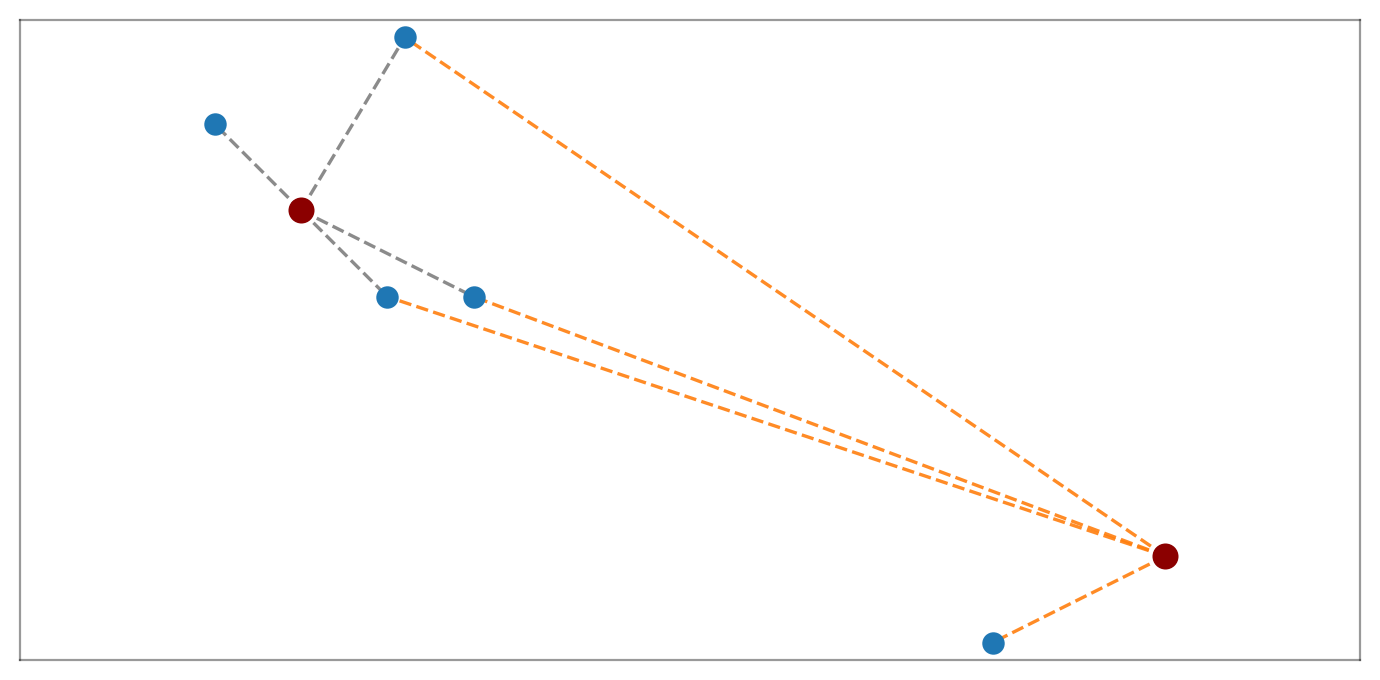
\includegraphics[width=0.5\linewidth]{dataset_python.png}
    \caption{The left red point has 4 ``good quality'' neighbors, while the right red point has only one close enough. Weighting this neighbor similarly to the points that are far apart hurts mean estimation.}
    \label{fig:placeholder}
\end{figure}

\subsubsection{Algorithm analysis}
Clearly $S_i(\epsilon)$ may not be uniquely defined (e.g there are more than $k$-points at most $\epsilon$ close to point i). We break these ties arbitrarily. 
\par Let $N_i^k$ be the set of the k-indices that are closest to point i. 
\begin{quote}
    \textbf{Adaptive opt.knn }must perfom at least as well as \textbf{opt.knn} for $\epsilon \leq  \max\limits_{i \in I}\max\limits_{j \in N_i^k} |x_i -x_j|$ (\textit{where $I$ is the set of points with missing coordinates}).
\end{quote}

\textbf{Proof of concept.} 
In $\text{opt.knn}$ we replace the missing coordinate of point $i$ with the average value of this coordinate over the $k$-closest neighbors of $i$. Clearly, this works well when the datapoints follow some common (unknown) distribution. As we pick closer neighbors we improve our estimation (by the Central Limit Theorem), while adding more distant neighbors increases noise in the estimation.

\par If we run $\text{opt.knn}$ we can then compute the maximum distance $R_i$ of any neighbor of point $i \in I$ from its $k$-closest neighbors. The maximum of these $R_i$'s defines a radius $r$, such that $\text{opt.knn}$ is equivalent to picking the $k$ points that are no more than $r$ away from any point $i \in I$. Hence it is clear that for
\[
\epsilon = \max_{i \in I} \max_{j \in N_i^k} \lVert x_i - x_j \rVert
\]
the two algorithms are equivalent.

\par Now observe that if the $R_i$'s are uniform then $\text{opt.knn}$ is optimal. However, if there are big differences between them we clearly hurt the estimation of points with smaller $R_i$ (points that have a coherent cluster of $k$ points around them). Our algorithm, though, uses $\text{opt.knn}$ on the subset of points that are $\epsilon$-close, but for the rest it weights them inversely to their distance. This allows for flexibility, depending on how good the neighbors are.


\begin{figure}[H]
    \centering
    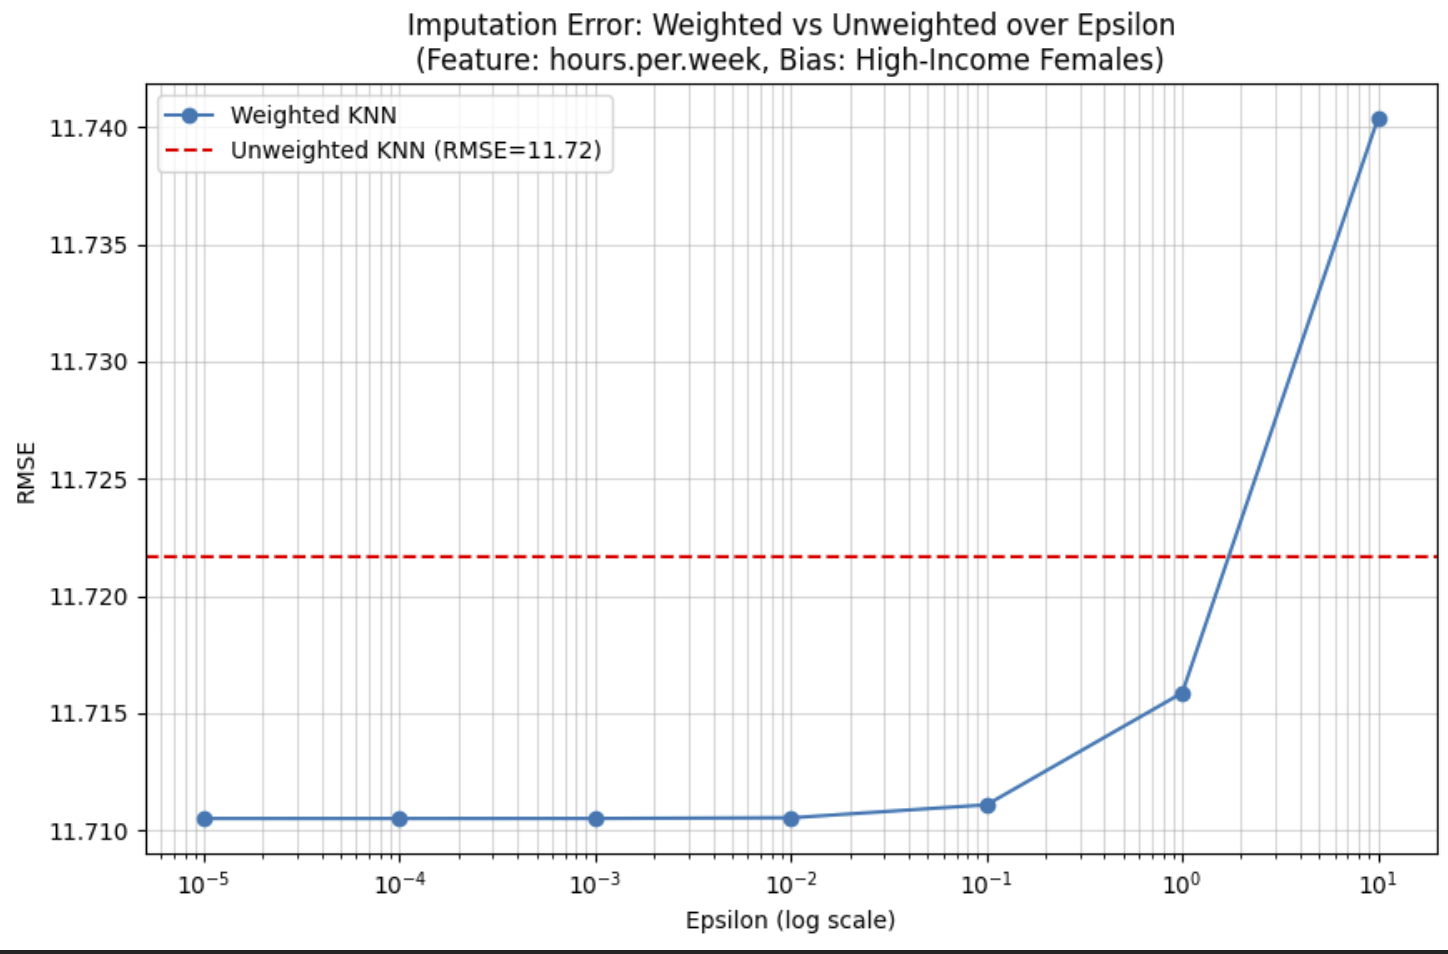
\includegraphics[width=0.5\linewidth]{varying_epsilon.png}
    \caption{RMSE error as $\epsilon$ varies}
    \label{fig:placeholder}
\end{figure}

\subsection{Case study: The \textbf{Adult} dataset} We use the \textsc{Adult} dataset from the UCI Machine Learning Repository, a standard benchmark for studying algorithmic fairness. The prediction task is to classify whether an individual's annual income exceeds \$50000. 
Among the available covariates, we choose to study as the protected attribute is \textit{sex}, with ``Female'' groups being significantly underrepresented among high-income individuals.  
\par We modify the dataset, by erasing form the column ``hours per week" (replacing with NaNs) rows that correspond to high-earning women. \\
\par We then detect rows that correspond to high-earning women (829 rows in total) and insert NaNs in the feature 'hours.per.week' in 580 out of the 829 of these rows.
Originally the dataset is biased in the sense that it contains fewer examples of high-earning women:
\begin{verbatim}
Counts of positive samples by sex:
sex
Male      6662
Female    1179
\end{verbatim}
We ran opt.knn for k =5 and k=8 as well as adaptive opt.knn. We got the following results:
\begin{verbatim}
Running opt.knn with k=5
--- Imputation Error for 'hours.per.week' ---
RMSE: 11.7217
MAE:  7.5838
Running opt.knn with k=8
--- Imputation Error for 'hours.per.week' ---
RMSE: 11.7002
MAE:  7.5827
Running opt.knn (adaptive) with k=5
--- Imputation Error for 'hours.per.week' ---
RMSE: 11.6947
MAE:  7.5262
\end{verbatim}
Focusing on the RMSE metric defined as :
\[
\mathrm{RMSE}
= \sqrt{\frac{1}{n}\sum_{i=1}^{n}\left(y_i - \hat{y}_i\right)^2}
\]
we observe that adaptive opt.knn achieves (modest) improvement. As the diagram above showed varying choosing $\epsilon \leq 10^{-2}$ achieved the best results.\\


\subsection{Future work}
It would be theoretically interesting to study how the initial bias of the dataset forms a lower bound on the bias of an imputation algorithm.
\par Another interesting direction is to examine the interplay between data imputation methods and synthetic data generation. In our view, when designing algorithms for synthetic data, it is important to account for the fairness properties of the datasets used for generation, so as to avoid scenarios in which synthetic data amplify the biases already present in the original data.

\section{In-Processing Approach: Fairness in Regression Models}

% ============================================================
% Robust / Stable Fair Regression (single adversary w)
% Fairness constraints: (1) Cov(f(X), d), (2) group mean parity,
% (3) group second-moment (variance) control (convex surrogate),
% (4) group MSE control (convex surrogate).
%
% Model: prediction \hat y_i = f_\theta(x_i), with f_\theta affine in \theta
% (e.g., linear regression). Sensitive d is discrete, observed only in training.
% ============================================================

\subsection{Analysis of Fairness Measure on Stable Regression}

% \subsubsection{Stable Regression}

\paragraph{Setting.}
We observe training data $\{(x_i,y_i,d_i)\}_{i=1}^n$, where $x_i\in\mathbb{R}^p$ are features,
$y_i\in\mathbb{R}$ is the target, and $d_i\in\{1,\dots,G\}$ is a discrete sensitive attribute.
The sensitive attribute $d$ is available during training but is \emph{not} used at prediction time.
Let $\mathcal{I}_g:=\{i:\ d_i=g\}$ be the index set of group $g$, with $n_g:=|\mathcal{I}_g|$. %and $\pi_g:=n_g/n$ the empirical group proportion.

We consider a prediction model $\hat y_i = f_\theta(x_i)$, parameterized by $\theta$.
To keep the overall optimization convex in $\theta$ (for fixed adversarial weights), we assume
$f_\theta(\cdot)$ is affine in $\theta$ (e.g., $f_\theta(x)=x^\top\beta+b$).

\paragraph{Stable Regression: adversary setting on residuals.}
Following the stable regression problem proposed by \cite{BertsimasPaskov2020}, we introduce an adversary that chooses a reweighting of the samples.
For a stability level $r\in(0,1]$ (ratio of data points to keep), define the standard Conditional Value at Risk (CVaR) weight set
\begin{equation}
\Delta_n^{(r)}
:=\left\{w\in\mathbb{R}^n:\ \sum_{i=1}^n w_i=r n,\ \ 0\le w_i \le 1\right\},
\label{eq:Walpha}
\end{equation}
where we would also use the alternative notation $\Delta_{n}^{(K)}$, where $K=\lfloor rn \rfloor$ (i.e, the exact number of samples to keep), when convenient.
This set restricts the adversary to focus on at most an $r$-fraction of the data (in a CVaR sense),
penalizing \emph{worst-case} behavior.

% \paragraph{Group-balance.}
% To prevent the adversary from ``hiding'' unfairness by allocating negligible mass to a minority group,
% we impose a group-balance constraint:
% \begin{equation}
% \sum_{i\in\mathcal{I}_g} w_i = \pi_g,\qquad g=1,\dots,G.
% \label{eq:groupbalance}
% \end{equation}
% We denote the resulting feasible set by
% \begin{equation}
% \mathcal{W}_{\alpha,\mathrm{bal}}
% :=\left\{w\in\mathcal{W}_\alpha:\ \sum_{i\in\mathcal{I}_g} w_i = \pi_g,\ \forall g\right\}.
% \label{eq:Wbal}
% \end{equation}

\paragraph{Stable LAD loss.}
We use the LAD (absolute deviation) loss:
\[
\ell_i(\theta) := |y_i - f_\theta(x_i)|.
\]
The stable regression loss is $\max_{w\in\mathcal{W}_{\alpha,\mathrm{bal}}}\sum_i w_i\ell_i(\theta)$,
which corresponds to a CVaR-type worst-case average of the LAD residuals.

\paragraph{Robust fairness penalties (all under the same adversary $w$).}
We aim to reduce dependence between predictions $\hat y$ and sensitive attribute $d$, and to control
group disparities in the prediction distribution and approximation error. Importantly,
\emph{all fairness terms are evaluated under the same adversarial weights $w$}, so the model is robust
``in every sense''.

We introduce four penalty weights
$\lambda_{\mathrm{cov}},\lambda_{\mu},\lambda_{\mathrm{var}},\lambda_{\mathrm{mse}}\ge 0$.
Setting any of them to $0$ effectively turns that penalty off.

\vspace{2mm}
\noindent\textbf{(1) Empirical covariance between prediction and sensitive attribute.}
For discrete $d$, we define a centered numeric coding $c_i:=d_i-\bar d$, where $\bar d:=\sum_{g=1}^G \pi_g g$
(the empirical mean of $d$). Under group-balance \eqref{eq:groupbalance}, $\bar d$ is fixed.
We then consider the weighted covariance proxy
\[
\mathrm{Cov}_w(\hat y,d) \;:=\; \sum_{i=1}^n w_i\,c_i\,\hat y_i,
\qquad \hat y_i=f_\theta(x_i).
\]
We penalize its absolute value.

\vspace{2mm}
\noindent\textbf{(2) First-moment parity (group mean matching).}
Define the weighted group mean prediction
\[
\mu_g(w,\theta)
:= \mathbb{E}_w[\hat y\mid d=g]
:= \frac{1}{\pi_g}\sum_{i\in\mathcal{I}_g} w_i\,\hat y_i.
\]
We penalize deviations from a common mean across groups via a worst-group bound:
$\max_g |\mu_g(w,\theta)-m|$ with an auxiliary scalar $m$.

\vspace{2mm}
\noindent\textbf{(3) Second-moment control (convex surrogate for variance parity).}
Exact constraints of the form $|\mathrm{Var}(\hat y\mid g)-\mathrm{Var}(\hat y\mid g')|$ are not convex.
Instead, we use a convex replacement: control the worst-group \emph{second central moment}.
Using the identity $\mathrm{Var}(Z)=\min_c \mathbb{E}[(Z-c)^2]$, we introduce per-group centers $c_g$ and penalize
\[
\max_{g}\ \frac{1}{\pi_g}\sum_{i\in\mathcal{I}_g} w_i\,(\hat y_i - c_g)^2.
\]
This is convex in $(\theta,\{c_g\})$ for fixed $w$.

\vspace{2mm}
\noindent\textbf{(4) Approximation-error parity (convex surrogate for MSE parity).}
Similarly, exact equality of group MSEs is nonconvex when written as a two-sided difference.
We instead bound the worst-group MSE:
\[
\max_{g}\ \frac{1}{\pi_g}\sum_{i\in\mathcal{I}_g} w_i\,\big(y_i-\hat y_i\big)^2,
\]
which is convex in $\theta$ for fixed $w$.


\subsection{A First Approach: Stable Regression with Covariance Constraint}

For simplicity, we focus on the case of a covariance constraint between the predicted value $f(X)$ and the sensitive attribute $d$. We explore two approaches for imposing this constraint: (i) directly imposing it on the original Stable Regression adversarial problem, and (ii) adding a penalty term that is also maximized on the inner problem of Stable Regression. That is, we explore the problems\\\\
\textbf{Naïve Covariance-Constrained Problem.}
{\everymath{\displaystyle}
\begin{align*}
    \begin{array}{rrll}
    \P_1(K, \varepsilon, \lambda):=&  \min_{\beta}  & \max_{w\in \Delta_{n}^{(K)}} \left\{ \sum_{i=1}^n w_i \cdot|y_i - x_i'\beta| \right\} + \lambda \mathcal{R}(\beta) &  \\
         & s.t. & \frac{1}{n}\left| \sum_{i=1}^n(d_i - \Bar{d})(\hat{y}_i - \overline{\hat{y}}) \right| \leq \varepsilon
    \end{array}
\end{align*}
\textbf{Surrogate Stable Covariance-Constrained Problem.}
\begin{align*}
    \begin{array}{rrll}
    \P_2(K, \rho, \lambda):=&  \min_{\beta} \max_{w\in \Delta_{n}^{(K)}} & \left\{ \sum_{i=1}^n w_i \cdot\left(|y_i - x_i'\beta| + \rho|(d_i - \Bar{d})(\hat{y}_i - \overline{\hat{y}})| \right)\right\} + \lambda \mathcal{R}(\beta), & \\
    =& \min_{\beta, \nu, \theta, u,\ell,c,q} \quad & K\nu + \sum_{i=1}^n \theta_i \\
    & s.t. \quad  & u_i + l_i + \rho (c_i + q_i) \leq \nu + \theta_i,& \forall i  \\
    &   & y_i - \hat{y}_i = u_i - \ell_i, & \forall i  \\
    && (d_i - \Bar{d})(\hat{y}_i - \overline{\hat{y}}) = c_i - q_i, & \forall i\\
   && 0 \leq \theta, u, \ell, c, q \\
   & & 
    \end{array}
\end{align*}}

\noindent where $\Bar{d}$ and $\overline{\hat{y}}$ represent the average of each quantity. The fundamental difference between the two approaches is that on the $\P_1$ we seek to satisfy the covariance constraint with all the samples on $X$ (keeping the same formulation as Stable Regression), whereas in $\P_2$ we only take into account, for the adversarial inner problem, the samples that are the most difficult to constrain, depending on the weight $\rho$ assigned to the covariance term in the objective. To be precise, to maintain the same procedure of Stable Regression and as a first approximation, in $\P_2$ we use a surrogate upper bound with the triangle inequality (i.e. $|a+b|\leq |a| + |b|$).

\paragraph{Min--max robust objective.}
One can extend the previous idea, combining stable LAD with the four robust fairness penalties, to solve:
\begin{equation}
\min_{\theta}\ \max_{w\in\mathcal{W}_{\alpha,\mathrm{bal}}}
\Bigg[
\sum_{i=1}^n w_i\,|y_i-f_\theta(x_i)|
\;+\;
\lambda_{\mathrm{cov}}\ \big|\mathrm{Cov}_w(\hat y,d)\big|
\;+\;
\lambda_{\mu}\ \Delta_\mu(w,\theta)
\;+\;
\lambda_{\mathrm{var}}\ \Delta_{\mathrm{var}}(w,\theta)
\;+\;
\lambda_{\mathrm{mse}}\ \Delta_{\mathrm{mse}}(w,\theta)
\Bigg]
\;+\;\lambda_{\mathrm{reg}}\mathcal{R}(\theta),
\label{eq:minmax_full}
\end{equation}
where $\mathcal{R}(\theta)$ is a convex regularizer (e.g., $\|\beta\|_1$ or $\tfrac12\|\beta\|_2^2$),
and the worst-group functionals are defined as
\begin{align*}
\Delta_\mu(w,\theta) &:= \max_{g} |\mu_g(w,\theta)-m| \quad (\text{with } m \text{ optimized}),\\
\Delta_{\mathrm{var}}(w,\theta) &:= \max_{g}\ \frac{1}{\pi_g}\sum_{i\in\mathcal{I}_g} w_i\,(\hat y_i - c_g)^2
\quad (\text{with } c_g \text{ optimized}),\\
\Delta_{\mathrm{mse}}(w,\theta) &:= \max_{g}\ \frac{1}{\pi_g}\sum_{i\in\mathcal{I}_g} w_i\,(y_i-\hat y_i)^2.
\end{align*}

\paragraph{Epigraph (upper-bounding) convex formulation.}
We rewrite \eqref{eq:minmax_full} using epigraph variables that upper bound each term.
Introduce scalars $\Gamma,\Delta,\Xi,H\ge 0$ and auxiliary variables $m\in\mathbb{R}$ and $c_g\in\mathbb{R}$.
Then \eqref{eq:minmax_full} is equivalent to:
\begin{equation}
\min_{\theta,\ m,\{c_g\}}
\ \max_{w\in\mathcal{W}_{\alpha,\mathrm{bal}},\ \Gamma,\Delta,\Xi,H\ge 0}
\left[
\sum_{i=1}^n w_i\,|y_i-f_\theta(x_i)|
+\lambda_{\mathrm{cov}}\,\Gamma
+\lambda_{\mu}\,\Delta
+\lambda_{\mathrm{var}}\,\Xi
+\lambda_{\mathrm{mse}}\,H
\right]
+\lambda_{\mathrm{reg}}\mathcal{R}(\theta),
\label{eq:minmax_epi}
\end{equation}
subject to the following convex upper-bounding constraints:
\begin{itemize}
\item \textbf{Covariance epigraph:}
\begin{equation}
\Gamma \;\ge\; \sum_{i=1}^n w_i\,c_i\,\hat y_i,
\qquad
\Gamma \;\ge\; -\sum_{i=1}^n w_i\,c_i\,\hat y_i,
\qquad \hat y_i=f_\theta(x_i).
\label{eq:cov_epi}
\end{equation}

\item \textbf{Mean-parity epigraph (worst-group deviation from common mean $m$):}
\begin{equation}
\Delta \;\ge\; \mu_g(w,\theta)-m,
\qquad
\Delta \;\ge\; -(\mu_g(w,\theta)-m),
\qquad \forall g,
\label{eq:mean_epi}
\end{equation}
where $\mu_g(w,\theta)=\frac{1}{\pi_g}\sum_{i\in\mathcal{I}_g} w_i \hat y_i$.

\item \textbf{Second-moment control epigraph (convex surrogate for variance parity):}
\begin{equation}
\Xi \;\ge\; \frac{1}{\pi_g}\sum_{i\in\mathcal{I}_g} w_i\,(\hat y_i - c_g)^2,
\qquad \forall g.
\label{eq:var_epi}
\end{equation}
This ensures no group has excessively large dispersion around its best-fitting center $c_g$.

\item \textbf{Worst-group MSE epigraph (convex surrogate for MSE parity):}
\begin{equation}
H \;\ge\; \frac{1}{\pi_g}\sum_{i\in\mathcal{I}_g} w_i\,(y_i-\hat y_i)^2,
\qquad \forall g.
\label{eq:mse_epi}
\end{equation}
This ensures no group has excessively large mean squared error.
\end{itemize}

\paragraph{Interpretation.}
The inner maximization over $w$ chooses a worst-case reweighting of at most an $\alpha$-fraction of the data
(in CVaR form), while maintaining group balance \eqref{eq:groupbalance}. Because the same $w$ appears in all
terms \eqref{eq:cov_epi}--\eqref{eq:mse_epi}, the adversary simultaneously stresses: (i) large LAD residuals,
(ii) dependence between $\hat y$ and $d$ via covariance, (iii) between-group differences in first moments of $\hat y$,
(iv) large within-group dispersion of predictions (a convex proxy for variance parity), and (v) large worst-group MSE.
The penalty weights $\lambda_{\mathrm{cov}},\lambda_\mu,\lambda_{\mathrm{var}},\lambda_{\mathrm{mse}}$
control which fairness notions are active and their relative strength.

\subsection{Case of Study: Results on the Student Dataset}

We analyze the first approach (Covariance Constraint) and the surrogate adversarial approach on the Student Dataset (\cite{studentperformance320}). Note that the performance of the Naive Covariance Approach consistently gets better results in that metric, while the Adversarial Surrogate gets consistently better in Accuracy Disparity and Variance, which makes sense with its form. This is a first approach, but already shows that there is room for improvement compared with baseline tree models, linear regression, and stable regression, as shown in the tables below.

\begin{figure}[!ht]
  \centering
  \begin{subfigure}{0.45\textwidth}
    \centering
    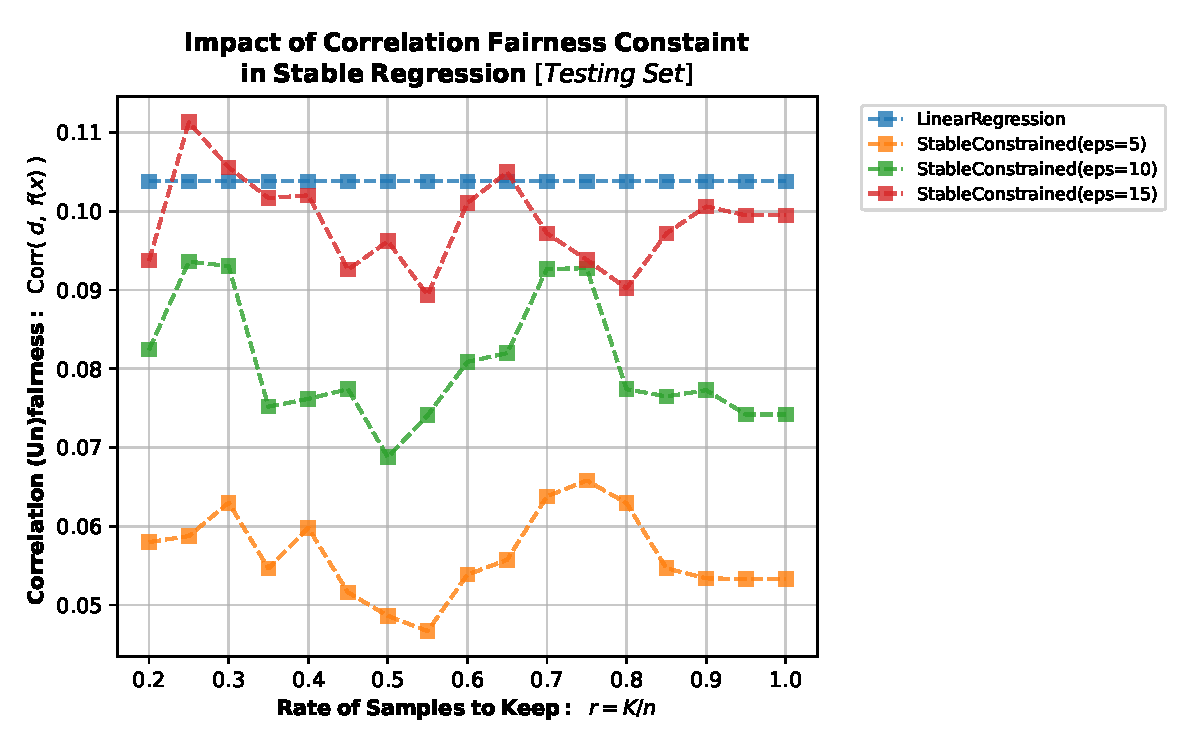
\includegraphics[width=\linewidth, trim={2cm 0.5cm 3.5cm 0cm}]{img/delete_vs_0_correlation_val.pdf}
    \caption{Linear Regression and $P_1(K,\varepsilon,\lambda)$, with $K=r\cdot n$ s.t. $r \in [0.2, 1]$, and $\varepsilon\in\{5,10,15\}$.}
    \label{fig:sub1}
  \end{subfigure}
  \hfill
  \begin{subfigure}{0.45\textwidth}
    \centering
    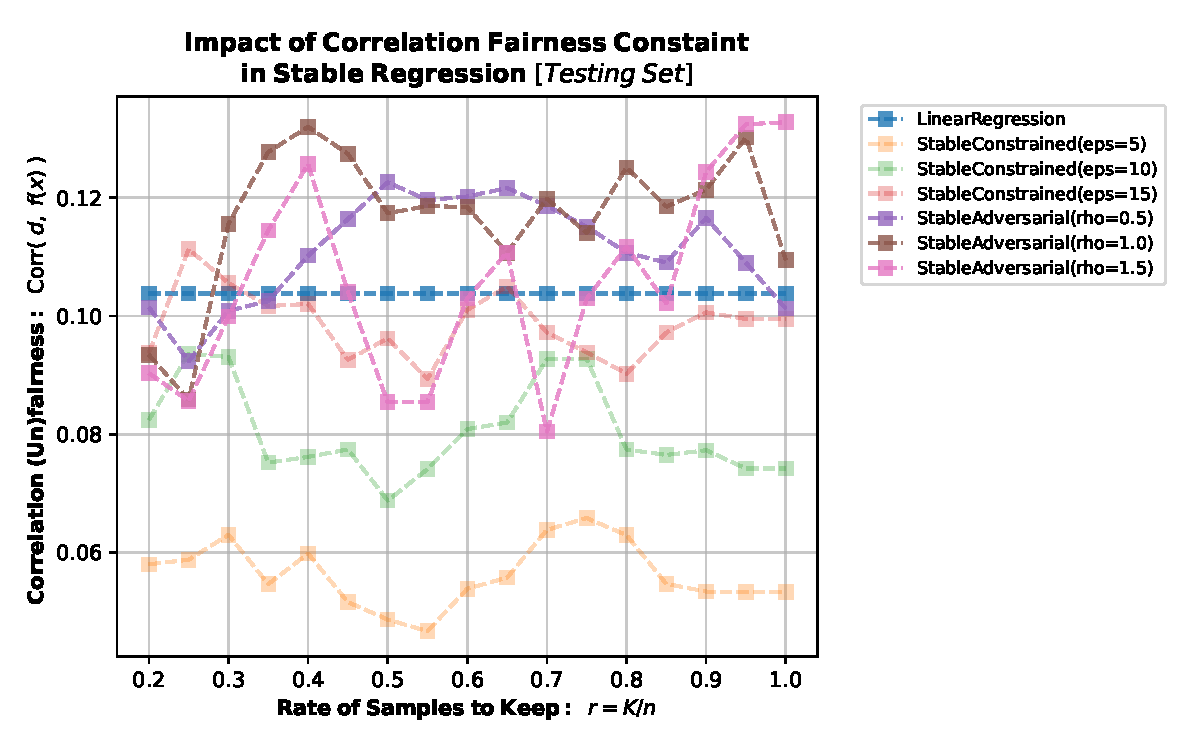
\includegraphics[width=\linewidth, trim={0cm 0.5cm 5cm 0cm}]{img/delete_vs_0_correlation_val_2.pdf}
    \caption{Same as (a), but adding $P_2(K,\rho,\lambda)$, with $K=r\cdot n$ s.t. $r \in [0.2, 1]$, and $\rho\in\{5,10,15\}$.}
    \label{fig:sub2}
  \end{subfigure}
  \caption{Behavior of Correlation (Un)fairness metric $Corr(d, f(X))$ (lower is better) for different models and ratio $r=K/n$ of data to keep, when constraining the covariance.}
  \label{fig:both}
\end{figure}


\begin{figure}[!ht]
  \centering
  \begin{subfigure}{0.45\textwidth}
    \centering
    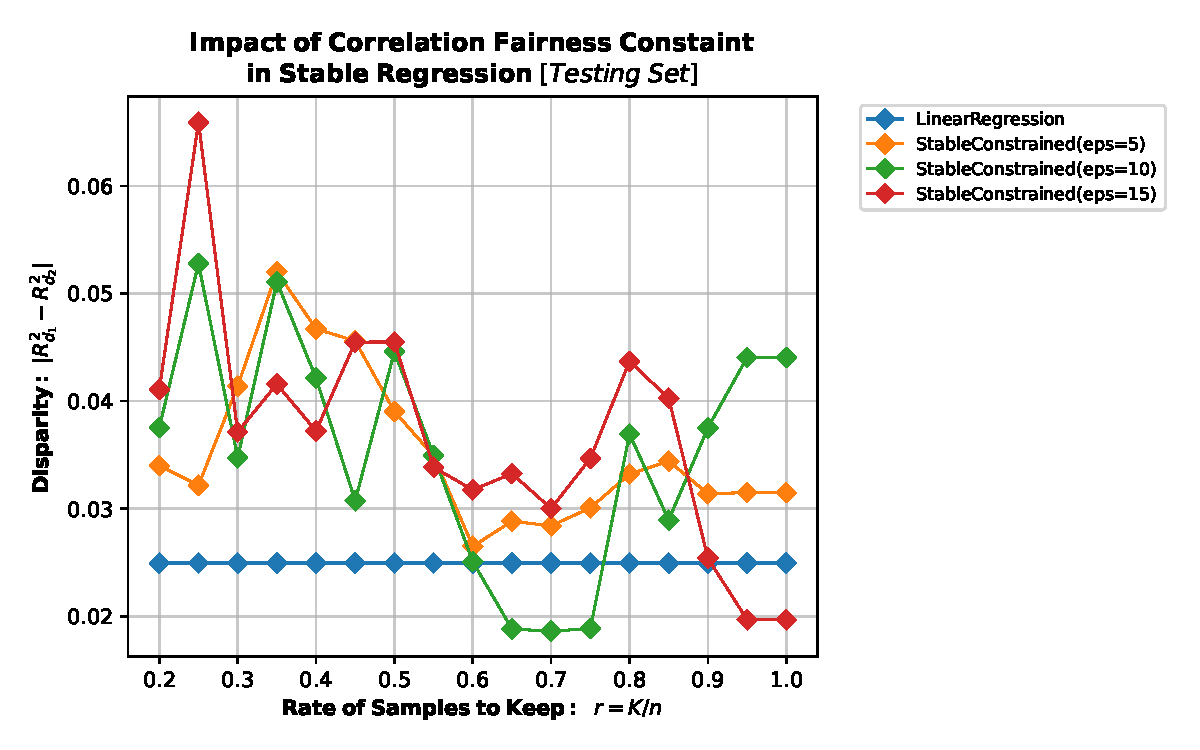
\includegraphics[width=\linewidth, trim={2cm 0.5cm 3.5cm 0cm}]{img/delete_vs_4_disparity.pdf}
    \caption{Linear Regression and $P_1(K,\varepsilon,\lambda)$, with $K=r\cdot n$ s.t. $r \in [0.2, 1]$, and $\varepsilon\in\{5,10,15\}$.}
    \label{fig:sub1}
  \end{subfigure}
  \hfill
  \begin{subfigure}{0.45\textwidth}
    \centering
    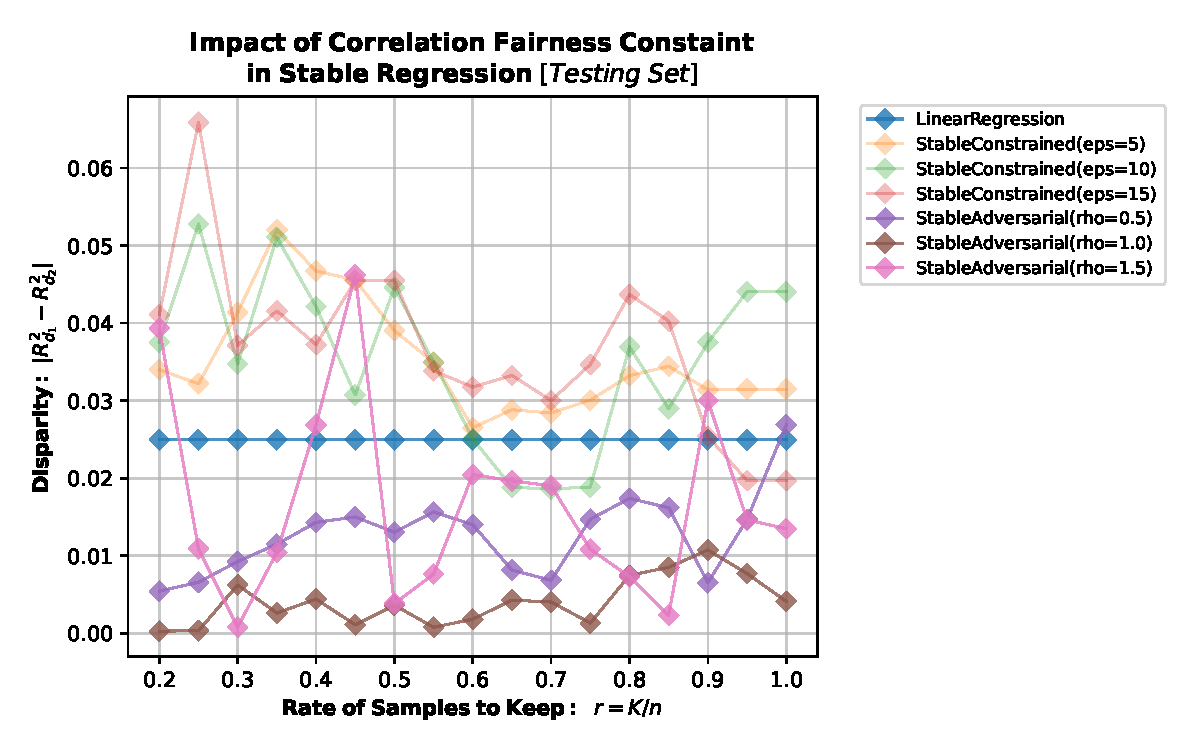
\includegraphics[width=\linewidth, trim={0cm 0.5cm 5cm 0cm}]{img/delete_vs_4_disparity_2.pdf}
    \caption{Same as (a), but adding $P_2(K,\rho,\lambda)$, with $K=r\cdot n$ s.t. $r \in [0.2, 1]$, and $\rho\in\{5,10,15\}$.}
    \label{fig:sub2}
  \end{subfigure}
  \caption{Behavior of Disparity metric $|R^2_{d_1} - R^2_{d_2}|$ (lower is better) for different models and ratio $r=K/n$ of data to keep, when constraining the covariance.}
  \label{fig:both}
\end{figure}


\begin{figure}[!ht]
  \centering
  \begin{subfigure}{0.45\textwidth}
    \centering
    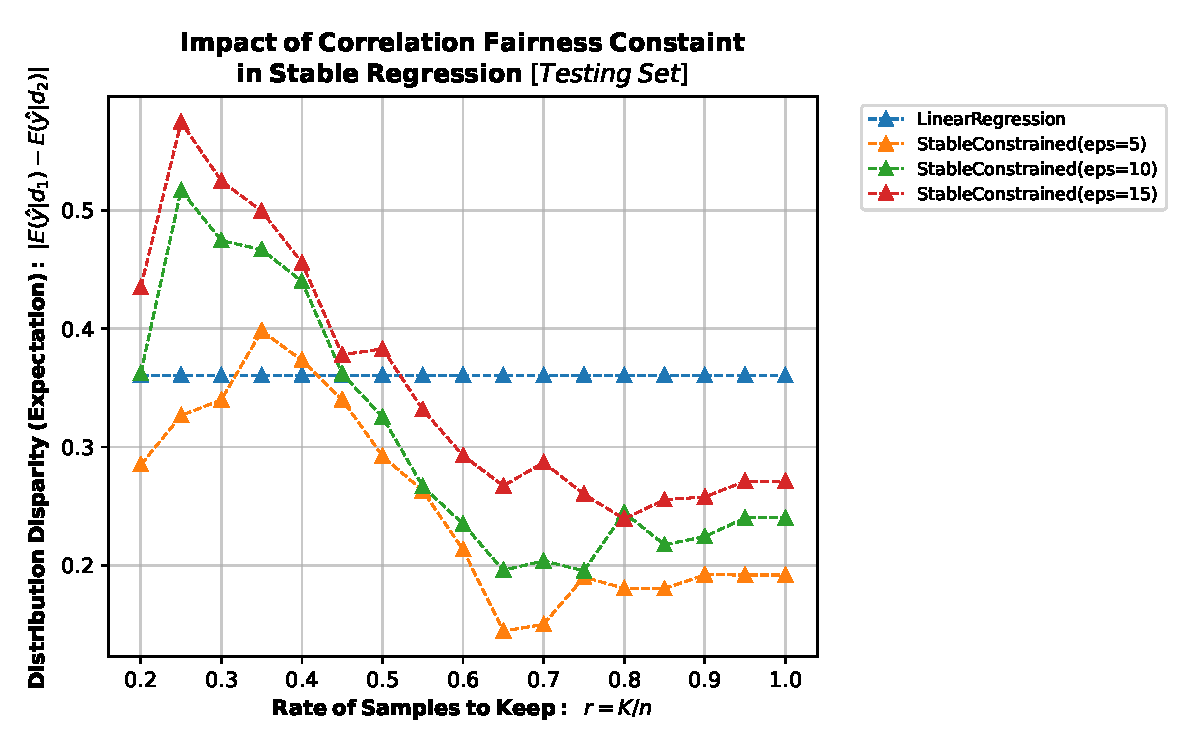
\includegraphics[width=\linewidth, trim={2cm 0.5cm 3.5cm 0cm}]{img/delete_vs_7_expected_f_X_val.pdf}
    \caption{Linear Regression and $P_1(K,\varepsilon,\lambda)$, with $K=r\cdot n$ s.t. $r \in [0.2, 1]$, and $\varepsilon\in\{5,10,15\}$.}
    \label{fig:sub1}
  \end{subfigure}
  \hfill
  \begin{subfigure}{0.45\textwidth}
    \centering
    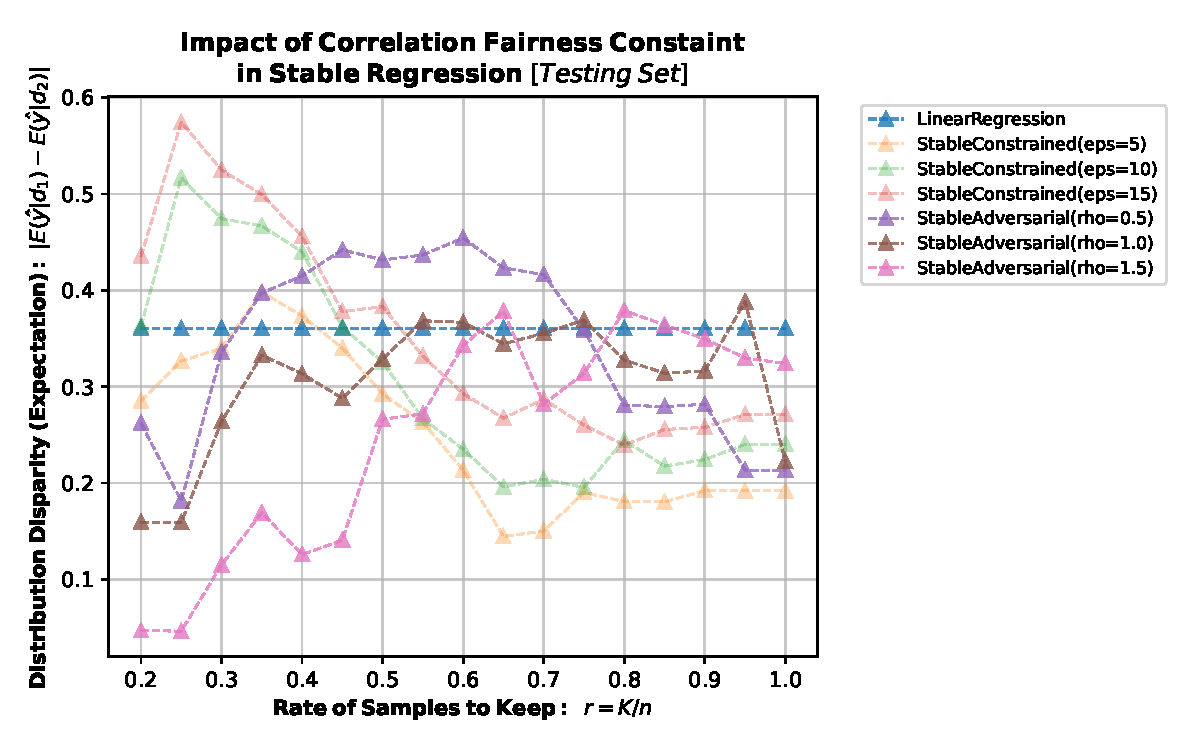
\includegraphics[width=\linewidth, trim={0cm 0.5cm 5cm 0cm}]{img/delete_vs_7_expected_f_X_val_2.pdf}
    \caption{Same as (a), but adding $P_2(K,\rho,\lambda)$, with $K=r\cdot n$ s.t. $r \in [0.2, 1]$, and $\rho\in\{5,10,15\}$.}
    \label{fig:sub2}
  \end{subfigure}
  \caption{Behavior of Disparity metric $|\mathbb{E}_{d_1} - \mathbb{E}_{d_2}|$ (lower is better) for different models and ratio $r=K/n$ of data to keep, when constraining the covariance.}
  \label{fig:both}
\end{figure}


\begin{figure}[!ht]
  \centering
  \begin{subfigure}{0.45\textwidth}
    \centering
    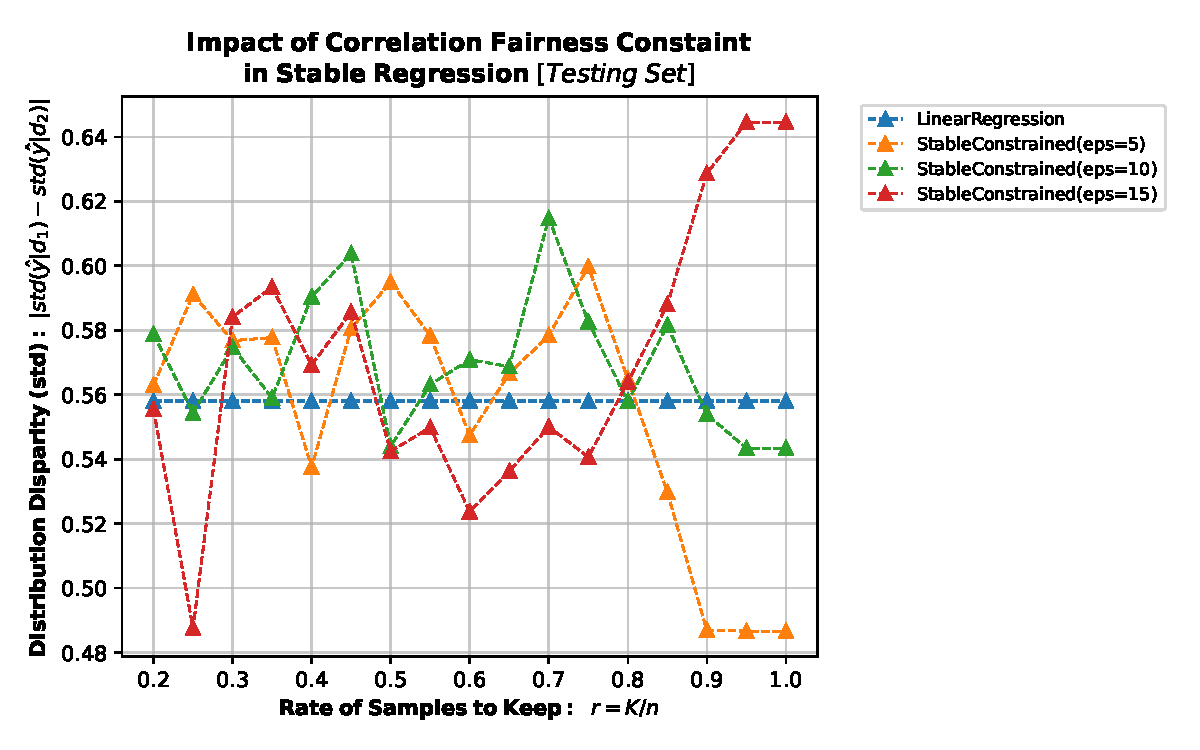
\includegraphics[width=\linewidth, trim={2cm 0.5cm 3.5cm 0cm}]{img/delete_vs_8_std_f_X_val.pdf}
    \caption{Linear Regression and $P_1(K,\varepsilon,\lambda)$, with $K=r\cdot n$ s.t. $r \in [0.2, 1]$, and $\varepsilon\in\{5,10,15\}$.}
    \label{fig:sub1}
  \end{subfigure}
  \hfill
  \begin{subfigure}{0.45\textwidth}
    \centering
    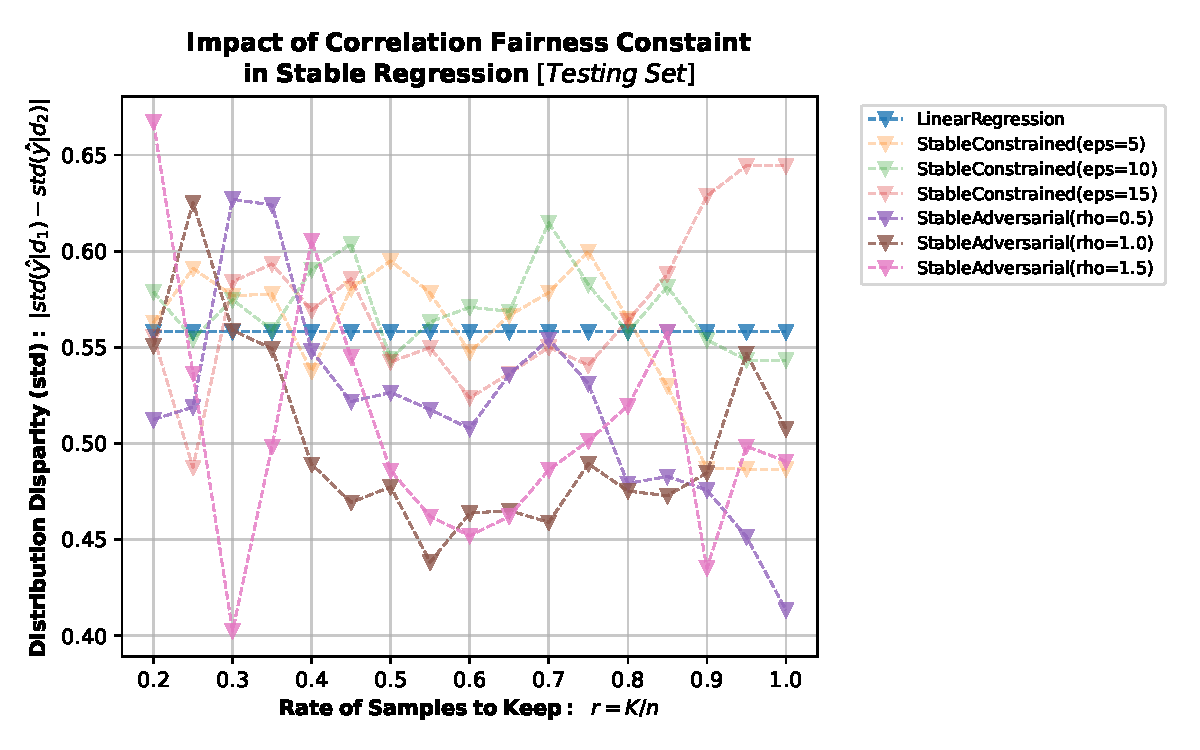
\includegraphics[width=\linewidth, trim={0cm 0.5cm 5cm 0cm}]{img/delete_vs_8_std_f_X_val_2.pdf}
    \caption{Same as (a), but adding $P_2(K,\rho,\lambda)$, with $K=r\cdot n$ s.t. $r \in [0.2, 1]$, and $\rho\in\{5,10,15\}$.}
    \label{fig:sub2}
  \end{subfigure}
  \caption{Behavior of Disparity metric $|std_{d_1} - std_{d_2}|$ (lower is better) for different models and ratio $r=K/n$ of data to keep, when constraining the covariance.}
  \label{fig:both}
\end{figure}



\begin{figure}[!ht]
  \centering
  \begin{subfigure}{0.45\textwidth}
    \centering
    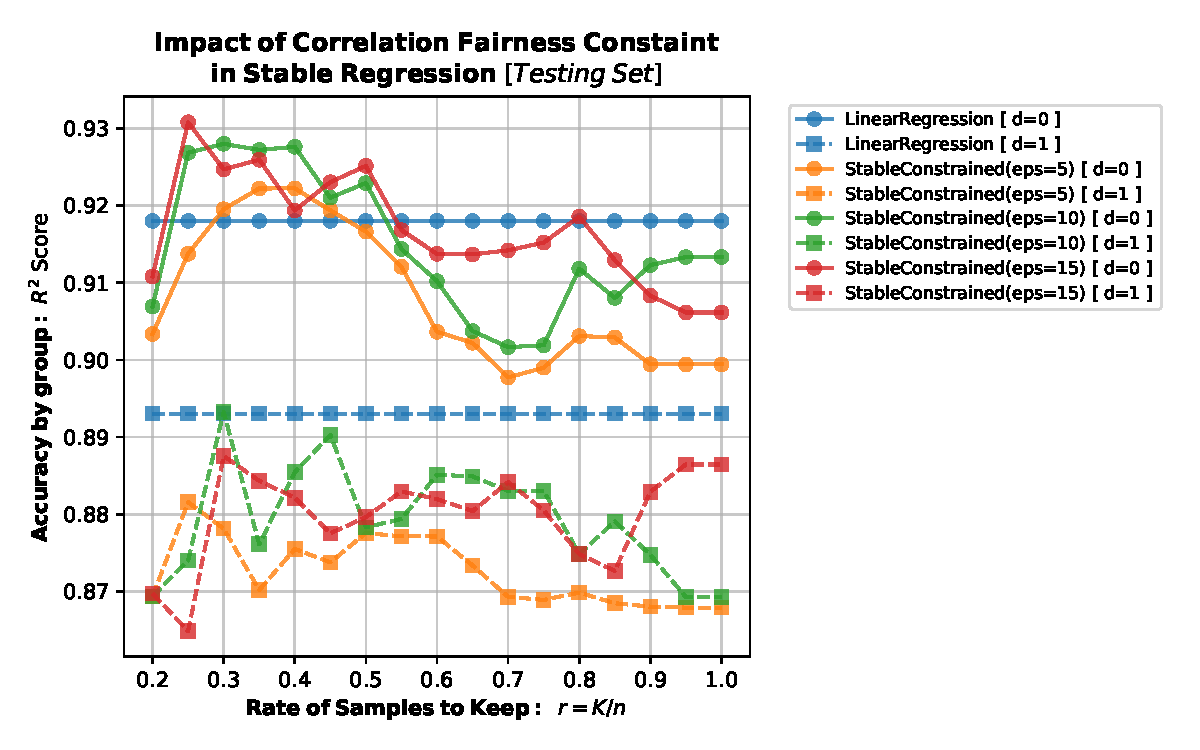
\includegraphics[width=\linewidth, trim={2cm 0.5cm 3.5cm 0cm}]{img/delete_vs_3_validation.pdf}
    \caption{Linear Regression and $P_1(K,\varepsilon,\lambda)$, with $K=r\cdot n$ s.t. $r \in [0.2, 1]$, and $\varepsilon\in\{5,10,15\}$.}
    \label{fig:sub1}
  \end{subfigure}
  \hfill
  \begin{subfigure}{0.45\textwidth}
    \centering
    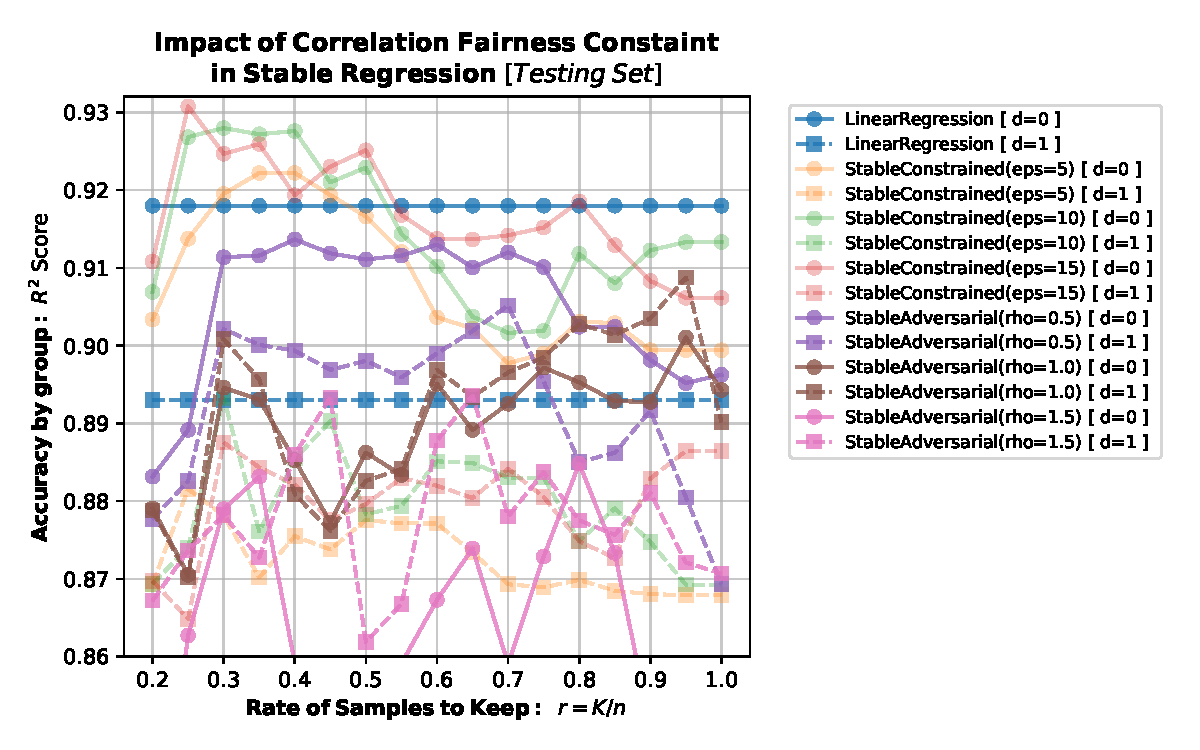
\includegraphics[width=\linewidth, trim={0cm 0.5cm 5cm 0cm}]{img/delete_vs_3_validation_2.pdf}
    \caption{Same as (a), but adding $P_2(K,\rho,\lambda)$, with $K=r\cdot n$ s.t. $r \in [0.2, 1]$, and $\rho\in\{5,10,15\}$.}
    \label{fig:sub2}
  \end{subfigure}
  \caption{Behavior of Disparity metric $|R^2_{d_1} - R^2_{d_2}|$ (lower is better) for different models and ratio $r=K/n$ of data to keep, when constraining the covariance.}
  \label{fig:both}
\end{figure}

% \begin{table}[!h]
% \caption{Model Performance Metrics}
% \label{tab:performance}
% \begin{tabular}{|l|c|r|r|r|r|r|}
% \toprule
%  & Parameters &\textbf{$R^2$ Score} & \textbf{$R^2$ Disp.} & \textbf{$|Corr(\hat{y}, d)|$} & \textbf{$\mathbb{E}$. Disp.} & \textbf{Std. Disp.} \\
% \midrule
% \textbf{RandomForest}      & - & 0.933 & 0.033 & 0.111 & 0.658 & 0.603 \\
% \textbf{GradientBoosting}  & - & 0.902 & 0.025 & 0.140 & 0.603 & 0.484 \\
% \textbf{ExtraTrees}        & - & \textbf{0.935} & 0.039 & 0.115 & 0.623 & 0.544 \\
% \textbf{LexicographicFair} & - & 0.903 & 0.029 & 0.115 & 0.285 & 0.645 \\
% \textbf{ProportionalFair}  & - & 0.902 & 0.030 & 0.114 & 0.281 & 0.648 \\
% \textbf{LADRegression}     & - & 0.902 & 0.031 & 0.113 & 0.274 & 0.646 \\
% \textbf{LinearRegression}  & - & 0.912 & 0.025 & 0.104 & 0.361 & 0.558 \\
% \midrule
% \textbf{StableConstrained} & $r=1.0,\varepsilon=10$ & 0.902 & 0.044 & \textbf{0.074} & 0.240 & 0.543 \\
% \textbf{StableConstrained} & $r=0.8,\varepsilon=10$ & 0.902 & 0.037 & 0.077 & 0.244 & 0.558 \\
% \textbf{StableConstrained} & $r=0.6,\varepsilon=10$ & 0.904 & 0.025 & 0.081 & 0.235 & 0.571 \\
% \textbf{StableConstrained} & $r=0.4,\varepsilon=10$ & 0.916 & 0.042 & 0.076 & 0.440 & 0.590 \\
% \textbf{StableAdversarial} & $r=1.0,\rho=0.1$& 0.895 & 0.004 & 0.110 & \textbf{0.222} & 0.508 \\
% \textbf{StableAdversarial} & $r=0.8,\rho=0.1$& 0.900 & 0.007 & 0.125 & 0.328 & 0.475 \\
% \textbf{StableAdversarial} & $r=0.6,\rho=0.1$& 0.898 & \textbf{0.002} & 0.118 & 0.367 & \textbf{0.464} \\
% \textbf{StableAdversarial} & $r=0.4,\rho=0.1$& 0.886 & 0.004 & 0.132 & 0.313 & 0.489 \\
% \bottomrule
% \end{tabular}
% \end{table}


\begin{table}[!h]
\caption{Model Performance Metrics}
\label{tab:performance}
\begin{tabular}{|l|c|r|r|r|r|r|}
\toprule
 &Parameters & \textbf{$R^2$ Score} & \textbf{$R^2$ Disp.} & \textbf{$|Corr(\hat{y}, d)|$} & \textbf{$\mathbb{E}$. Disp.} & \textbf{Std. Disp.} \\
\midrule
\textbf{RandomForest}     & - & 0.933 & 0.033 & 0.111 & 0.658 & 0.603 \\
\textbf{GradientBoosting} & - & 0.902 & 0.025 & 0.140 & 0.603 & 0.484 \\
\textbf{ExtraTrees}       & - & \textbf{0.935} & 0.039 & 0.115 & 0.623 & 0.544 \\
\textbf{LADRegression}    & - & 0.902 & 0.031 & 0.113 & 0.274 & 0.646 \\
\textbf{LinearRegression} & - & 0.912 & 0.025 & 0.104 & 0.361 & 0.558 \\
\textbf{StableRegression} & $r=1.0$ & 0.901 & 0.030 & 0.112 & 0.269 & 0.656 \\
\textbf{StableRegression} & $r=0.8$ & 0.908 & 0.039 & 0.099 & 0.290 & 0.587 \\
\textbf{StableRegression} & $r=0.6$ & 0.906 & 0.047 & 0.101 & 0.310 & 0.488 \\
\textbf{StableRegression} & $r=0.4$ & 0.912 & 0.036 & 0.112 & 0.486 & 0.574 \\
\midrule
\textbf{StableConstrained} &$r=1.0,\varepsilon=10$ & 0.902 & 0.044 & \textbf{0.074} & 0.240 & 0.543 \\
\textbf{StableConstrained} &$r=0.8,\varepsilon=10$ & 0.902 & 0.037 & 0.077 & 0.244 & 0.558 \\
\textbf{StableConstrained} &$r=0.6,\varepsilon=10$ & 0.904 & 0.025 & 0.081 & 0.235 & 0.571 \\
\textbf{StableConstrained} &$r=0.4,\varepsilon=10$ & 0.916 & 0.042 & 0.076 & 0.440 & 0.590 \\
\textbf{StableAdversarial} &$r=1.0,\rho=0.1$ & 0.895 & 0.004 & 0.110 & \textbf{0.222} & 0.508 \\
\textbf{StableAdversarial} &$r=0.8,\rho=0.1$ & 0.900 & 0.007 & 0.125 & 0.328 & 0.475 \\
\textbf{StableAdversarial} &$r=0.6,\rho=0.1$ & 0.898 & \textbf{0.002} & 0.118 & 0.367 & \textbf{0.464} \\
\textbf{StableAdversarial} &$r=0.4,\rho=0.1$ & 0.886 & 0.004 & 0.132 & 0.313 & 0.489 \\
\bottomrule
\end{tabular}
\end{table}


% \begin{table}[!h]
% \caption{Percentage Difference vs LinearRegression}
% \label{tab:performance_diff}
% \begin{tabular}{|l|c|r|r|r|r|r|}
% \toprule
%  & Parameters & \textbf{$R^2$ Score} & \textbf{$R^2$ Disp.} & \textbf{$|Corr(\hat{y}, d)|$} & \textbf{$\mathbb{E}$. Disp.} & \textbf{Std. Disp.} \\
% \midrule
% \textbf{RandomForest}      & - & +2.30\% & +32.00\% & +6.73\% & +82.27\% & +8.06\% \\
% \textbf{GradientBoosting}  & - & -1.10\% & +0.00\% & +34.62\% & +67.04\% & -13.26\% \\
% \textbf{ExtraTrees}        & - & \textbf{+2.52\%} & +56.00\% & +10.58\% & +72.58\% & -2.51\% \\
% \textbf{LexicographicFair} & - & -0.99\% & +16.00\% & +10.58\% & -21.05\% & +15.59\% \\
% \textbf{ProportionalFair}  & - & -1.10\% & +20.00\% & +9.62\% & -22.16\% & +16.13\% \\
% \textbf{LADRegression}     & - & -1.10\% & +24.00\% & +8.65\% & -24.10\% & +15.77\% \\
% \textbf{LinearRegression}  & - & +0.00\% & +0.00\% & +0.00\% & +0.00\% & +0.00\% \\
% \midrule
% \textbf{StableConstrained} & $r=1.0,\varepsilon=10$ & -1.10\% & +76.00\% & \textbf{-28.85\%} & -33.52\% & -2.69\% \\
% \textbf{StableConstrained} & $r=0.8,\varepsilon=10$ & -1.10\% & +48.00\% & -25.96\% & -32.41\% & +0.00\% \\
% \textbf{StableConstrained} & $r=0.6,\varepsilon=10$ & -0.88\% & +0.00\% & -22.12\% & -34.90\% & +2.33\% \\
% \textbf{StableConstrained} & $r=0.4,\varepsilon=10$ & +0.44\% & +68.00\% & -26.92\% & +21.88\% & +5.73\% \\
% \textbf{StableAdversarial} & $r=1.0,\rho=0.1$ & -1.86\% & -84.00\% & +5.77\% & \textbf{-38.50\%} & -8.96\% \\
% \textbf{StableAdversarial} & $r=0.8,\rho=0.1$ & -1.32\% & -72.00\% & +20.19\% & -9.14\% & -14.87\% \\
% \textbf{StableAdversarial} & $r=0.6,\rho=0.1$ & -1.54\% & \textbf{-92.00\%} & +13.46\% & +1.66\% & \textbf{-16.85\%} \\
% \textbf{StableAdversarial} & $r=0.4,\rho=0.1$ & -2.85\% & -84.00\% & +26.92\% & -13.30\% & -12.37\% \\
% \bottomrule
% \end{tabular}
% \end{table}


\begin{table}[!h]
\caption{Percentage Difference vs LinearRegression}
\label{tab:performance_diff}
\begin{tabular}{|l|c|r|r|r|r|r|}
\toprule
 & Parameters & \textbf{$R^2$ Score} & \textbf{$R^2$ Disp.} & \textbf{$|Corr(\hat{y}, d)|$} & \textbf{$\mathbb{E}$. Disp.} & \textbf{Std. Disp.} \\
\midrule
\textbf{RandomForest}     & - & +2.30\% & +32.00\% & +6.73\% & +82.27\% & +8.06\% \\
\textbf{GradientBoosting} & - & -1.10\% & +0.00\% & +34.62\% & +67.04\% & -13.26\% \\
\textbf{ExtraTrees}       & - & \textbf{+2.52\%} & +56.00\% & +10.58\% & +72.58\% & -2.51\% \\
\textbf{LADRegression}    & - & -1.10\% & +24.00\% & +8.65\% & -24.10\% & +15.77\% \\
\textbf{LinearRegression} & - & +0.00\% & +0.00\% & +0.00\% & +0.00\% & +0.00\% \\
\textbf{StableRegression} & $r=1.0$ & -1.21\% & +20.00\% & +7.69\% & -25.48\% & +17.56\% \\
\textbf{StableRegression} & $r=0.8$ & -0.44\% & +56.00\% & -4.81\% & -19.67\% & +5.20\% \\
\textbf{StableRegression} & $r=0.6$ & -0.66\% & +88.00\% & -2.88\% & -14.13\% & -12.54\% \\
\textbf{StableRegression} & $r=0.4$ & +0.00\% & +44.00\% & +7.69\% & +34.63\% & +2.87\% \\
\midrule
\textbf{StableConstrained} & $r=1.0,\varepsilon=10$ & -1.10\% & +76.00\% & \textbf{-28.85\%} & -33.52\% & -2.69\% \\
\textbf{StableConstrained} & $r=0.8,\varepsilon=10$ & -1.10\% & +48.00\% & -25.96\% & -32.41\% & +0.00\% \\
\textbf{StableConstrained} & $r=0.6,\varepsilon=10$ & -0.88\% & +0.00\% & -22.12\% & -34.90\% & +2.33\% \\
\textbf{StableConstrained} & $r=0.4,\varepsilon=10$ & +0.44\% & +68.00\% & -26.92\% & +21.88\% & +5.73\% \\
\textbf{StableAdversarial} & $r=1.0,\rho=0.1$& -1.86\% & -84.00\% & +5.77\% & \textbf{-38.50\%} & -8.96\% \\
\textbf{StableAdversarial} & $r=0.8,\rho=0.1$& -1.32\% & -72.00\% & +20.19\% & -9.14\% & -14.87\% \\
\textbf{StableAdversarial} & $r=0.6,\rho=0.1$& -1.54\% & \textbf{-92.00\%} & +13.46\% & +1.66\% & \textbf{-16.85\%} \\
\textbf{StableAdversarial} & $r=0.4,\rho=0.1$& -2.85\% & -84.00\% & +26.92\% & -13.30\% & -12.37\% \\
\bottomrule
\end{tabular}
\end{table}




\section{Conclusions}
In this work, we explored the behavior of several optimization-based methods (e.g., OptKNN and stable regression) commonly used in machine learning through the lens of fairness. In particular, we demonstrated that, with small and carefully designed modifications, these methods can be adapted to simultaneously optimize predictive performance and mitigate unfair outcomes affecting minority groups. 
However, our results also highlight that the observed improvements are highly sensitive to 
\begin{enumerate}
    \item the specific definition of ``fairness,''
    \item the choice of ``sensitive'' group,
    \item the characteristics of the dataset under consideration.
\end{enumerate}
This sensitivity underscores the context-dependent nature of fairness interventions.
\par Consequently we believe that: 
\begin{quote}
\textit{There is no single method that is inherently biased. Rather, bias emerges from a combination of factors, including properties of the dataset, algorithmic design choices, and the selection of optimization objectives. }
\end{quote}
Addressing unfairness therefore requires a holistic approach that accounts for these interacting sources, rather than relying on a one-size-fits-all solution.

% \bibliography{references}
\printbibliography
\end{document}
